%%%%%%%%%%%%%%%%%%%%%%%%%%%%%%%%%%%%%%%%%
% Beamer Presentation
% LaTeX Template
% Version 2.0 (March 8, 2022)
%
% This template originates from:
% https://www.LaTeXTemplates.com
%
% Author:
% Vel (vel@latextemplates.com)
%
% License:
% CC BY-NC-SA 4.0 (https://creativecommons.org/licenses/by-nc-sa/4.0/)
%
%%%%%%%%%%%%%%%%%%%%%%%%%%%%%%%%%%%%%%%%%

%%%%%%%%%%%%%%%%%%%%%%%%%%%%%%%%%%%%%%%%%
% This presentation template is an adaptation of the template mentioned above. It has been created by Giovanni Spadaro and it is available on GitHub (https://github.com/Giovo17/presentation-template-unict-lm-data).
%%%%%%%%%%%%%%%%%%%%%%%%%%%%%%%%%%%%%%%%%
    
%----------------------------------------------------------------------------------------
%	PACKAGES AND OTHER DOCUMENT CONFIGURATIONS
%----------------------------------------------------------------------------------------

\documentclass[
	11pt, % Set the default font size, options include: 8pt, 9pt, 10pt, 11pt, 12pt, 14pt, 17pt, 20pt
	%t, % Uncomment to vertically align all slide content to the top of the slide, rather than the default centered
	%aspectratio=169, % Uncomment to set the aspect ratio to a 16:9 ratio which matches the aspect ratio of 1080p and 4K screens and projectors
]{beamer}

\graphicspath{{img/}} % Specifies where to look for included images (trailing slash required)

\usepackage{booktabs} % Allows the use of \toprule, \midrule and \bottomrule for better rules in tables
\usepackage{parskip} 
%----------------------------------------------------------------------------------------
%	SELECT LAYOUT THEME
%----------------------------------------------------------------------------------------

% Beamer comes with a number of default layout themes which change the colors and layouts of slides. Below is a list of all themes available, uncomment each in turn to see what they look like.

\usetheme{Boadilla}

%----------------------------------------------------------------------------------------
%	SELECT COLOR THEME
%----------------------------------------------------------------------------------------

% Definição de cores personalizadas
\definecolor{primaryColor}{RGB}{20,45,105}
\definecolor{secondaryColor}{RGB}{0,100,160}

% Aplicação das cores no tema
\setbeamercolor{structure}{fg=primaryColor}
\setbeamercolor{palette primary}{bg=primaryColor, fg=white}
\setbeamercolor{palette secondary}{bg=secondaryColor, fg=white} 
\setbeamercolor{title}{bg=secondaryColor, fg=white}
\setbeamercolor{block title}{bg=secondaryColor, fg=white}
\setbeamercolor{block body}{bg=secondaryColor!10, fg=black}

\usetheme{Boadilla}

%----------------------------------------------------------------------------------------
%	SELECT FONT THEME & FONTS
%----------------------------------------------------------------------------------------

% Beamer comes with several font themes to easily change the fonts used in various parts of the presentation. Review the comments beside each one to decide if you would like to use it. Note that additional options can be specified for several of these font themes, consult the beamer documentation for more information.

\usefonttheme{default} % Typeset using the default sans serif font
%\usefonttheme{serif} % Typeset using the default serif font (make sure a sans font isn't being set as the default font if you use this option!)
%\usefonttheme{structurebold} % Typeset important structure text (titles, headlines, footlines, sidebar, etc) in bold
%\usefonttheme{structureitalicserif} % Typeset important structure text (titles, headlines, footlines, sidebar, etc) in italic serif
%\usefonttheme{structuresmallcapsserif} % Typeset important structure text (titles, headlines, footlines, sidebar, etc) in small caps serif

%------------------------------------------------

%\usepackage{mathptmx} % Use the Times font for serif text
\usepackage{palatino} % Use the Palatino font for serif text

%\usepackage{helvet} % Use the Helvetica font for sans serif text
\usepackage[default]{opensans} % Use the Open Sans font for sans serif text
%\usepackage[default]{FiraSans} % Use the Fira Sans font for sans serif text
%\usepackage[default]{lato} % Use the Lato font for sans serif text

%----------------------------------------------------------------------------------------
%	SELECT INNER THEME
%----------------------------------------------------------------------------------------
\useinnertheme{circles}


%---------------------------------------------------------------------------------------
%	SELECT OUTER THEME
%----------------------------------------------------------------------------------------

\useoutertheme{miniframes}
\setbeamertemplate{navigation symbols}{} % Uncomment this line to remove the navigation symbols from the bottom of all slides

%----------------------------------------------------------------------------------------
%	PRESENTATION INFORMATION
%----------------------------------------------------------------------------------------

\title[MAP2310]{Uma análise numérica do atrator de Lorenz}
\author[TAYLOR, L. A.; LIMA, J. C. M.]{Lucas Amaral Taylor \and Julio Cezar de Moura Lima}
\institute[IME-USP]{
    Instituto de Matemática e Estatística da Universidade de São Paulo - USP}
\date[2024]{Junho de 2024}

%----------------------------------------------------------------------------------------

\begin{document}

%----------------------------------------------------------------------------------------
%	TITLE SLIDE
%----------------------------------------------------------------------------------------

\begin{frame}

        \begin{figure}
		
\includegraphics[width=0.4\linewidth]{img/logo_v2.png}
	\end{figure}
 
	\titlepage % Output the title slide, automatically created using the text entered in the PRESENTATION INFORMATION block above
\end{frame}

%----------------------------------------------------------------------------------------
%	TABLE OF CONTENTS SLIDE
%----------------------------------------------------------------------------------------

% The table of contents outputs the sections and subsections that appear in your presentation, specified with the standard \section and \subsection commands. You may either display all sections and subsections on one slide with \tableofcontents, or display each section at a time on subsequent slides with \tableofcontents[pausesections]. The latter is useful if you want to step through each section and mention what you will discuss.

\begin{frame}
	\frametitle{Estrutura da apresentação} % Slide title, remove this command for no title
	
	\tableofcontents % Output the table of contents (all sections on one slide)
	%\tableofcontents[pausesections] % Output the table of contents (break sections up across separate slides)
\end{frame}

%----------------------------------------------------------------------------------------
%	PRESENTATION BODY SLIDES
%----------------------------------------------------------------------------------------



\section{Introdução} 


%------------------------------------------------

\begin{frame}
    \frametitle{O fenômeno de convecção atmosférica}

    Segundo Charles A. Doswell III, meteorologista americano, o fenômeno de convecção atmosférica, pode ser definido como:

    \vspace{1em} % Adiciona um espaço vertical de 1em

    \begin{quote}
        \itshape
        ``De um modo geral, a convecção refere-se ao transporte de uma determinada propriedade através do movimento de um fluido, na maioria das vezes com referência ao transporte de calor''
    \end{quote}

    \begin{flushright}
        \tiny
        \textit{Fonte: Doswell III, C. A., \textbf{Severe Convective Storms}, American Meteorological Society, 1996.}
    \end{flushright}
\end{frame}
%------------------------------------------------

\begin{frame}
    \frametitle{\textit{Finite Amplitude Free Convection as an Initial Value Problem—I}}
    
    Em 1962, Barry Saltzman publica o artigo que intitula este slide. Nele, Saltzman realiza experimentos meteorológicos e hidrodinâmicos. O artigo, tem dois objetivos:
    \vspace{0.5em}
    \begin{enumerate}
        \item Formular um modelo matemático para fenômenos de convecção de natureza não-linear;
        
        \item Determinar um método de solução de um caso de movimento convectivo dependente do tempo bidimensionais.
    \end{enumerate}
\end{frame}

%------------------------------------------------

\begin{frame}[t]
    \frametitle{\small Equação desenvolvida por Saltzman}
    
    {\small
    \begin{equation}
        \frac{a}{(1 + a^2)^k} \psi = x(t)\sqrt{2} \sin \left(\frac{\pi u}{a}\right) \sin \left(\frac{\pi v}{H}\right)
    \end{equation}
    \begin{equation}
        \frac{\pi R_o \theta}{R \Delta T} = y(t)\sqrt{2} \cos \left(\frac{\pi u}{a}\right) \sin \left(\frac{\pi v}{H}\right) - z(t) \sin \left(\frac{2\pi}{H}v\right)
    \end{equation}
    }

    {\scriptsize
    Onde:
    \begin{itemize}
        \item $u$: coordenada espacial horizontal ($m$);
        \item $x(t), y(t), z(t)$: coeficientes dependentes do tempo (amplitudes) (Unidade depende do contexto);
        \item $\frac{\pi}{H}$: inverso da profundidade da camada de fluido (máximo de $v$) ($m^{-1}$);
        \item $a$: parâmetro de geometria;
        \item $Ra$: número de Rayleigh;
        \item $R_c$: valor crítico de $Ra$ ($R_c = \pi^4(1 + a^2)^3/a^2$);
        \item $\Delta T$: diferença de temperatura total ($K$).
    \end{itemize}
    }
\end{frame}
%------------------------------------------------

\begin{frame}[t]
    \frametitle{Equação desenvolvida por Lorenz}
    \scriptsize
    Lorenz simplificou a equação desenvolvida por Saltzman, eliminou as funções trigonométricas e adotou equações diferenciais ordinárias. Temos o seguinte resultado:

    \begin{align*}
        \begin{cases}
            \dfrac{dx}{dt} &= \sigma(y-x) \\[6pt]
            \dfrac{dy}{dt} &= x(\rho - z) - y \\[6pt]
            \dfrac{dz}{dt} &= xy - \beta z
        \end{cases}
    \end{align*}

    \vspace{0.2cm}

    \begin{itemize}
        \item $\sigma$ controla a sensibilidade do sistema à diferença entre as variáveis $x$ e $y$ (número de Prandtl). 
        \item $\rho$ está associado à taxa de convecção do sistema (número de Rayleigh).
        \item $\beta$ está associado à geometria do sistema e à diferença entre as taxas de crescimento das variáveis $x$ e $z$.
    \end{itemize}
\end{frame}
    
%------------------------------------------------
\section{Tratamento Numérico}

\begin{frame}
    \frametitle{Abordagem}
    \begin{enumerate}
        \item Utilizamos o método \textit{Runge-Kutta} para a \textbf{discretização} e \textbf{resolução do sistema de equações diferenciais};
        \item Empregamos \textit{splines cúbicas} para a \textbf{representação gráfica};
        \item Aplicamos o \textit{Método dos Mínimos Quadrados (MMQ)} para a \textbf{análise da sensibilidade} do sistema.
    \end{enumerate}
        
        

\end{frame}

%------------------------------------------------

\begin{frame}
    \frametitle{Razões para a seleção do Método Runge-Kutta}
    Optamos pelo Método de Runge-Kutta pelos seguinte motivos:
    \begin{enumerate}
        \item O método escolhido calcula inclinações em quatro pontos dentro de cada intervalo de tempo, oferecendo uma aproximação mais precisa em comparação aos métodos aprendidos em aula.

        \item O método de quarta ordem possui um erro de truncamento local da ordem de $h^5$ e um erro de truncamento global da ordem de $h^4$, onde $h$ é o passo de tempo.
    \end{enumerate}
\end{frame}

%------------------------------------------------
\begin{frame}
    \frametitle{Método Runge-Kutta}

    Para as nossas simulações, os valores dos parâmetros utilizados são:

    \begin{block}{Parâmetros do sistema}
        \centering
        $\sigma = 10, \quad \rho = 28, \quad \beta = 8/3$
    \end{block}

    \begin{block}{Condições iniciais}
        \centering
        $x_0 = 0, \quad y_0 = 1, \quad z_0 = 1.05$
    \end{block}

    \begin{block}{Configurações do método}
        \centering
        Passo de tempo: $h = 0.01, \quad \text{Número de passos} = 1 \times 10^4$
    \end{block}

\end{frame}



%------------------------------------------------

\begin{frame}
    \frametitle{Evolução do atrator em função do número de passos}
    \begin{figure}[htbp]
        \centering
        \begin{minipage}{0.32\textwidth}
            \centering
            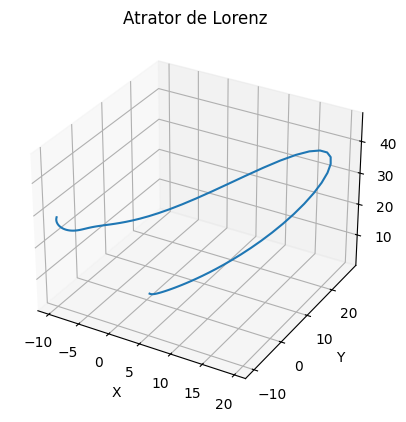
\includegraphics[width=\linewidth]{01_docs/00_Relatorio/img/attrator100.png}
            \vspace{0.5em} % Espaço para ajuste visual
            {\scriptsize $1 \times 10^2$ passos}
        \end{minipage}\hfill
        \begin{minipage}{0.32\textwidth}
            \centering
            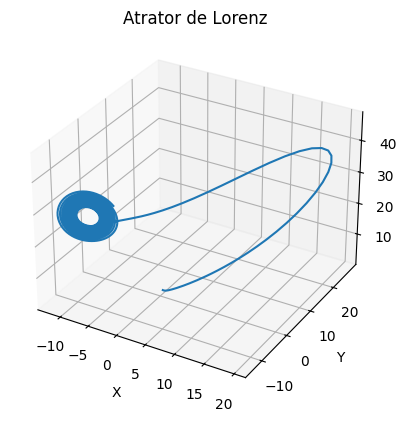
\includegraphics[width=\linewidth]{01_docs/00_Relatorio/img/attrator1000.png}
            \vspace{0.5em} % Espaço para ajuste visual
            {\scriptsize $1 \times 10^3$ passos}
        \end{minipage}\hfill
        \begin{minipage}{0.32\textwidth}
            \centering
            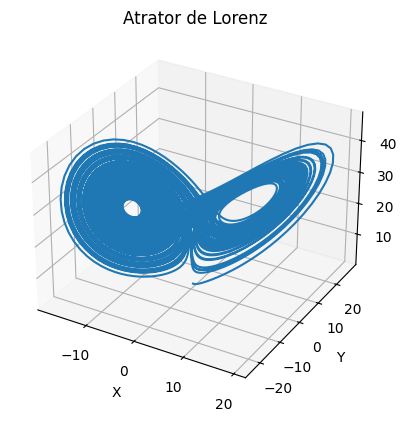
\includegraphics[width=\linewidth]{01_docs/00_Relatorio/img/attrator10000.png}
            \vspace{0.5em} % Espaço para ajuste visual
            {\scriptsize $1 \times 10^4$ passos}
        \end{minipage}
    \end{figure}
\end{frame}


%------------------------------------------------

\begin{frame}
    \frametitle{Justificativa do emprego de \textit{Spline} cúbicas}
    \begin{enumerate}
        \item Garantia de suavidade e continuidade nas curvas, essenciais dada a natureza não-linear e caótica do sistema. 
        \item Métodos, como o de Lagrange, não são adequados devido à perda de informação decorrente da linearização, comprometendo a representação precisa do sistema.
    \end{enumerate}
\end{frame}

%------------------------------------------------

\begin{frame}
    \frametitle{\textit{Spline} Cúbicas: resultado obtidos}      
    
    \begin{figure}
        \centering
        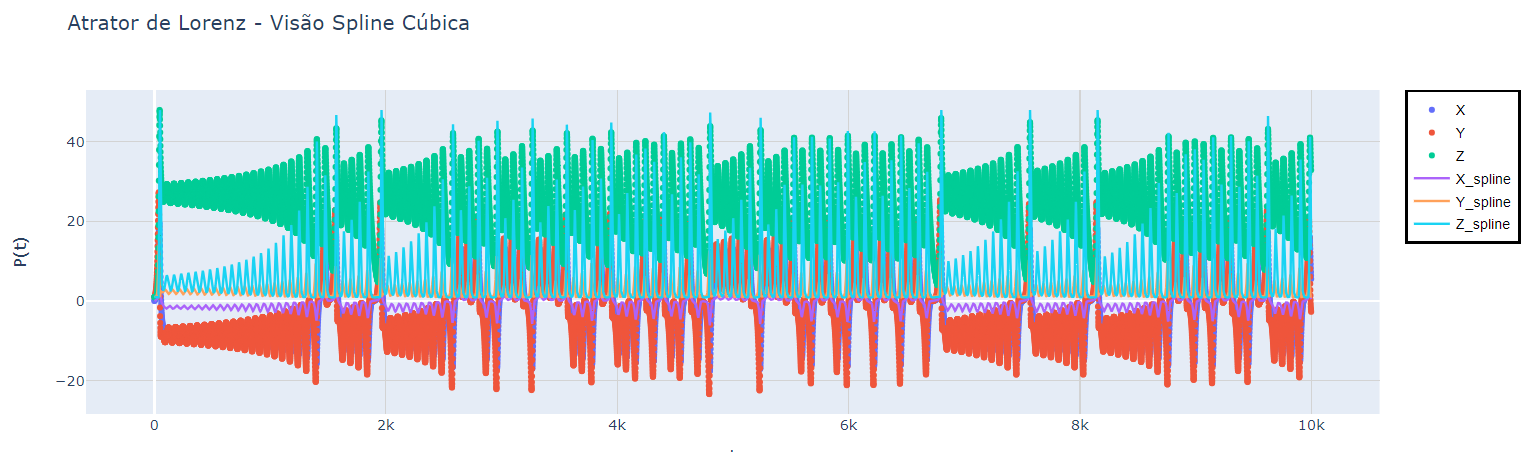
\includegraphics[width=1.0\textwidth]{01_docs/00_Relatorio/img/spline.png}
    \end{figure}

    \vspace{0.2cm}

    \begin{center}
        {\tiny Produzido pelos autores}
    \end{center}
    
\end{frame}
%------------------------------------------------

\begin{frame}
    \frametitle{Motivos para a adoção do MMQ}
    \begin{enumerate}
        \item O MMQ aproxima bem as dinâmicas não-lineares do sistema.
        \item Quantifica o impacto das alterações nos parâmetros e como pequenas mudanças afetam o sistema.
        \item Destaca-se pela alta eficiência computacional.
    \end{enumerate}
\end{frame}

%------------------------------------------------

\begin{frame}
    \frametitle{MMQ: Resultados obtidos}
    \begin{figure}
        \centering
        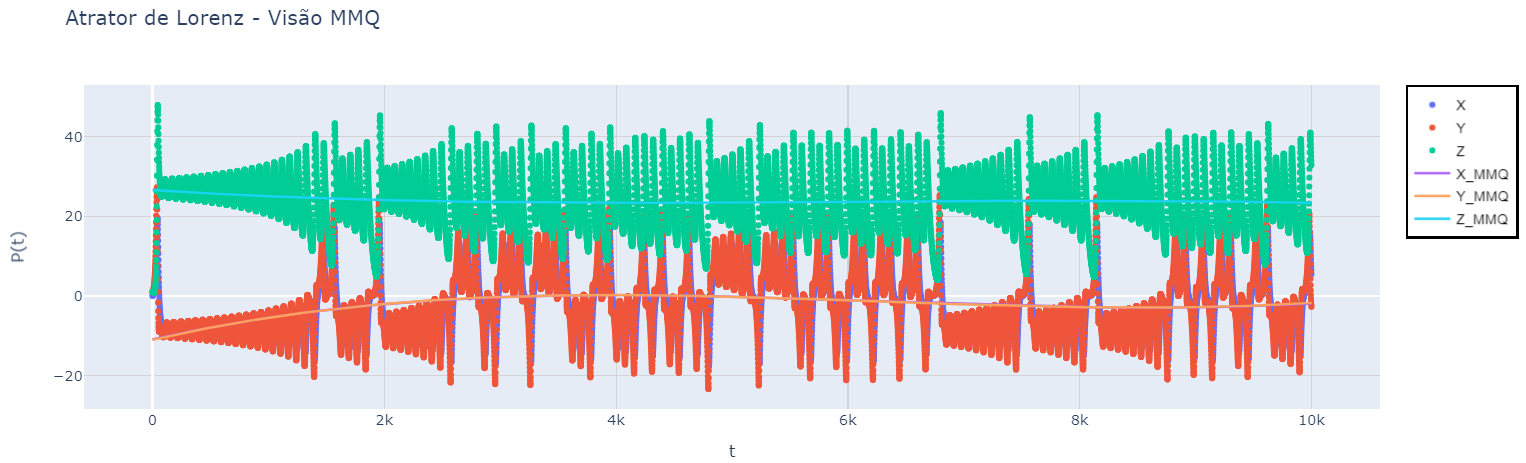
\includegraphics[width=1.0\textwidth]{01_docs/00_Relatorio/img/mmq.png}
    \end{figure}

    \vspace{0.2cm}

        \begin{center}
        {\tiny Produzido pelos autores}
    \end{center}
    
\end{frame}


\section{Erro e convergência}

\begin{frame}
    \frametitle{Abordagem para o Tratamento do Erro}
    \begin{enumerate}
        \item O atrator de Lorenz não possui uma \textbf{solução analítica}.
        \item Usamos a \textbf{solução numérica} com o menor $h$ como referência ``\textbf{exata}''.
        \item O \textbf{erro} é a diferença entre as soluções numéricas para diferentes $h$ e essa referência.
    \end{enumerate}
\end{frame}


%------------------------------------------------

\begin{frame}
    \frametitle{Tabela de Convergência no método RK4}
    \scriptsize
    \begin{table}[H]
    \centering
    \begin{tabular}{c c c c c c c c c c}
    \toprule
     & $X_{0.01}$ & $Y_{0.01}$ & $Z_{0.01}$ & $X_{0.001}$ & $Y_{0.001}$ & $Z_{0.001}$ & $X_{0.0001}$ & $Y_{0.0001}$ & $Z_{0.0001}$ \\
    \midrule
    0  & 0.000 & 1.000 & 1.050 & 0.000 & 1.000 & 1.050 & 0.000 & 1.000 & 1.050 \\
    1  & 0.095 & 1.003 & 1.023 & 0.010 & 0.999 & 1.047 & 0.001 & 1.000 & 1.050 \\
    2  & 0.183 & 1.031 & 0.997 & 0.020 & 0.999 & 1.044 & 0.002 & 1.000 & 1.049 \\
    3  & 0.266 & 1.081 & 0.973 & 0.030 & 0.998 & 1.042 & 0.003 & 1.000 & 1.049 \\
    4  & 0.346 & 1.152 & 0.951 & 0.039 & 0.998 & 1.039 & 0.004 & 1.000 & 1.049 \\
    5  & 0.427 & 1.245 & 0.931 & 0.049 & 0.998 & 1.036 & 0.005 & 1.000 & 1.049 \\
    6  & 0.511 & 1.359 & 0.912 & 0.058 & 0.999 & 1.034 & 0.006 & 1.000 & 1.048 \\
    7  & 0.598 & 1.495 & 0.896 & 0.068 & 0.999 & 1.031 & 0.007 & 1.000 & 1.048 \\
    8  & 0.691 & 1.653 & 0.882 & 0.077 & 1.000 & 1.028 & 0.008 & 0.999 & 1.048 \\
    9  & 0.791 & 1.837 & 0.872 & 0.086 & 1.002 & 1.025 & 0.009 & 0.999 & 1.047 \\
    \bottomrule
    \end{tabular}
    \caption{Tabela de Convergência no método RK4}
    \end{table}
\end{frame}

%------------------------------------------------

%------------------------------------------------

\begin{frame}
    \frametitle{Diferenças \(\Delta X\), \(\Delta Y\), \(\Delta Z\) no método RK4}
    \scriptsize % ou \tiny para uma fonte ainda menor
    \begin{table}[H]
    \centering
    \begin{tabular}{c c c c c c c c c}
    \toprule
     & \multicolumn{3}{c}{\(\Delta\) entre \(0.01\) e \(0.001\)} & & \multicolumn{3}{c}{\(\Delta\) entre \(0.01\) e \(0.0001\)} \\
    \cmidrule{2-4} \cmidrule{6-8}
     & \(\Delta X\) & \(\Delta Y\) & \(\Delta Z\) & & \(\Delta X\) & \(\Delta Y\) & \(\Delta Z\) \\
    \midrule
    0  & 0.000 & 0.000 & 0.000 & & 0.000 & 0.000 & 0.000 \\
    1  & 0.085 & 0.004 & -0.024 & & 0.094 & 0.003 & -0.027 \\
    2  & 0.163 & 0.032 & -0.047 & & 0.181 & 0.031 & -0.052 \\
    3  & 0.236 & 0.083 & -0.069 & & 0.263 & 0.081 & -0.076 \\
    4  & 0.307 & 0.154 & -0.088 & & 0.342 & 0.152 & -0.098 \\
    5  & 0.378 & 0.247 & -0.105 & & 0.422 & 0.245 & -0.118 \\
    6  & 0.453 & 0.360 & -0.122 & & 0.505 & 0.359 & -0.136 \\
    7  & 0.530 & 0.496 & -0.135 & & 0.591 & 0.495 & -0.151 \\
    8  & 0.614 & 0.653 & -0.146 & & 0.683 & 0.653 & -0.166 \\
    9  & 0.705 & 0.835 & -0.153 & & 0.782 & 0.838 & -0.175 \\
    \bottomrule
    \end{tabular}
    \caption{Diferenças entre os valores de \(X\), \(Y\) e \(Z\) para diferentes passos de integração}
    \end{table}
\end{frame}


%------------------------------------------------


\begin{frame}
    \frametitle{Convergência do Erro no Método RK4}
    \begin{itemize}
        \item \textbf{Redução do Erro com Passos Menores}: Passos menores no RK4 resultam em valores mais precisos. As diferenças \(\Delta X\), \(\Delta Y\) e \(\Delta Z\) diminuem à medida que o passo de integração é reduzido. 
        \item \textbf{Convergência do Método RK4}: Passos menores mostram que o RK4 converge para a solução correta. Os valores de \(X\), \(Y\) e \(Z\) tornam-se mais próximos com passos menores.
    \end{itemize}
        
\end{frame}
%------------------------------------------------
\section{Conclusão}
%------------------------------------------------

\begin{frame}{Principais referências}
    \footnotesize
    \begin{thebibliography}{99}
        \bibitem{Lorenz1963}
            E. N. Lorenz,
            \textit{Deterministic Nonperiodic Flow},
            Journal of the Atmospheric Sciences,
            1963, 20(2), pp. 130-141,
            \href{https://doi.org/10.1175/1520-0469(1963)020<0130:DNF>2.0.CO;2}{doi:10.1175/1520-0469(1963)020<0130:DNF>2.0.CO;2}
            
        \bibitem{ford1933}
            L. R. Ford,
            \textit{Differential Equations},
            McGraw-Hill,
            1955
            
        \bibitem{burden2016}
            R. L. Burden, D. J. Faires, A. M. Burden,
            \textit{Análise Numérica},
            Editora Cengage,
            2016
            
        \bibitem{roma2023}
            A. M. Roma, J. S. Bevilacqua, R. L. Nós,
            \textit{Métodos para a solução numérica de equações diferenciais ordinárias a valores iniciais},
            Notas de aula, curso de Métodos Numéricos, USP,
            2023
            
        \bibitem{peitgen2013}
            Heinz-Otto Peitgen, Hartmut J{\"u}rgens, Dietmar Saupe,
            \textit{Chaos and Fractals},
            Springer Science \& Business Media,
            2013
            
    \end{thebibliography}
\end{frame}


%------------------------------------------------




%----------------------------------------------------------------------------------------
%	CLOSING SLIDE


\begin{frame}

    
    \begin{center}
        \huge{Obrigado!}
    \end{center}
\end{frame}

%----------------------------------------------------------------------------------------
%----------------------------------------------------------------------------------------

\end{document} 